% !TEX root = ../thesis.tex

\chapter{Learning Arbitrary Sequences of Candidate Explanations}
\label{sec:nn}

In Section~\ref{sec:cn} we have presented an approach for generating candidate explanations in a fixed given order. However, as we cannot assume that humans generate candidates in a static sequence, having an approach which is more abstract and can learn arbitrary sequences would be the ideal scenario. Therefore, in this chapter we will focus on recurrent networks, more specifically in Jordan and Elman networks. We will show how these networks can be used to archive the same results presented for the previous approach, but also how they can easily be generalised for arbitrary sequences.

\section{Non-Complementary Candidate Explanations}
\label{sec:nn:ncce}

In Section~\ref{sec:cn} we have shown by means of an example how a predefined sequence of non-complementary candidate explanations can be generated based on connectionist networks. Now we would like to start this section by showing that the same result can also be archived based on recurrent networks. In order to do so, we will begin by constructing, training and testing a recurrent network for the same example used before. Thus, reconsider the program $\CalP_{sup}$ presented in Example~\ref{example:suppression} on page ~\pageref{example:suppression}.

In the first version of the connectionist network presented before, each of the nine candidate explanations is generated one after the other in a fixed order. After generating the last one, unit \Done is activated and the network returns to its initial state. Every time a new candidate explanation is generated, the state of the network remains the same until a next candidate is requested by the activation of unit \textit{next}. This means that the expected output is the previous candidate explanation when unit \textit{next} is passive and the next one, otherwise.

One possible way to translate this problem into a temporal domain problem is by constructing a sequence of binary vectors consisting of five bits. The first four bits (from left to right) will correspond to the four output units of the connectionist network, representing $e^\top$, $e^\bot$, $t^\top$ and $t^\bot$. The last bit (from left to right) corresponds to unit \Done of the connectionist network, representing whether all the non-complementary candidate explanations have been generated. Each of these bits will be equal to \textit{one} when its respective unit is active and equal to \textit{zero} when it is passive.

Given this, there are different sequences we could obtain depending on the oscillation of the values of the request unit \textit{next}. As explained in Chapter~\ref{sec:cn}, we are just working with one component of a network which generated the sceptical consequences of a given program $\CalP$ and observation $\CalO$. Therefore, the activation of unit \textit{next} will come from the other components of this overall network which is responsible for checking weather a given candidate explanation $\CalC$ explains $\CalO$ given $\CalP$.

If we consider the scenario where the network only needs one time step to decide whether the candidate was an explanation, then next candidates would be requested one after another without a break. In that case we have the most basic sequence, which is the request sequence where unit \textit{next} is active for nine time steps in a row. For this sequence of values for the request unit, the output sequence expected is the following: 
\[
00000, 10000, 01000, 00100, 00010, 10100, 10010, 01100, 01011.
\]

However, this is not always the case since we don't know how many time steps the external network will need before requesting a next candidate explanation. Moreover, this steps are not fixed, meaning that for different candidates it might take a different number of time steps. Therefore, we can also obtain any sequence which has the following form: 
\[
\begin{array}{lllll}
(00000)^+,&(10000)^+, &(01000)^+, &(00100)^+, &(00010)^+,\\
	        &(10100)^+, &(10010)^+, &(01100)^+, &(01011)^+.
\end{array}
\]

The main task here is to predict, at each point in time, the next binary vector in the sequence which represents the next candidate explanation. The value of this vector will depend on two factors: the last candidate explanation generated and the value of unit \textit{next}. Thus, our input will also consist of a 5-bit binary vector where the first four bits (from left to right) also correspond to $e^\top$, $e^\bot$, $t^\top$ and $t^\bot$, but the last bit (from left to right) corresponds to unit \textit{next} of the connectionist network, representing the request of a new candidate explanation. This bit will be equal to \textit{one} when a new candidate explanation should be generated and \textit{zero}, otherwise. All possible inputs and its respective expected outputs can be seen in Table~\ref{table:trainingexplanations}.

\begin{table}
		\centering
	\begin{subtable}[h]{0.30\textwidth}
		\centering
		\begin{tabular}{cc}
		Input & Output \\
		\hline
		00000 & 00000 \\
		10000 & 10000 \\
		01000 & 01000 \\
		00100 & 00100 \\
		00010 & 00010 \\
		10100 & 10100 \\
		10010 & 10010 \\
		01100 & 01100 \\
		01010 & 01011 \\
		\end{tabular}
		\bigskip
		\caption{Cases where the fifth bit in the input is \textit{zero}.}
		\label{table:trainingexplanations:zero}
	\end{subtable}
	\hspace{2cm}
	\begin{subtable}[h]{0.30\textwidth}
		\centering
		\begin{tabular}{cc}
		Input & Output \\
		\hline
		00001 & 10000 \\
		10001 & 01000 \\
		01001 & 00100 \\
		00101 & 00010 \\
		00011 & 10100 \\
		10101 & 10010 \\
		10011 & 01100 \\
		01101 & 01011 \\
		01011 & 00000 \\
		\end{tabular}
		\bigskip
		\caption{Cases where the fifth bit in the input is \textit{one}.}
		\label{table:trainingexplanations:one}
	\end{subtable}
	\caption{Each possible input and its respective expected output represented as 5-bit binary vectors for the generation of non-complementary candidate explanations for the given program $\CalP_{sup}$.}
	\label{table:trainingexplanations}
\end{table}

Now we would like to define a recurrent network corresponding to the behaviour described above. Since we are dealing with a temporal domain problem, the most suitable type of network in our case would be a recurrent network. As discussed in Section~\ref{sec:preliminaries}, there are many different types of recurrent networks but here we will focus only on two of them, which are the Jordan and the Elman networks. The Elman network is an variation of the Jordan network and the only difference between them is in the source of the connections to the context layer. In an Elman network, the connections to the context units come from the hidden units instead of the output units as it is done in a Jordan network. Because of this, it is clear that the input and output specifications described above can be equally applied for both types of networks.

When it comes to the structure of the network, the 5-bit binary vector input described above can be mapped into the input layer of the network where each bit corresponds to a unit. Thus, the input layer consists of five units. The same applies to the output layer which will then also consist of five units. As mentioned before, these two layers are exactly the same for both the Elman and the Jordan network. On the other hand, the context layer has different dependencies in each case. For the Jordan network, the context layer is a copy of the output layer and, thus, also has five units. But in the Elman network, the context layer is a copy of the hidden layer. If we consider a hidden layer of size five, then the context layer of the Elman network would also consist of five units. The structure of the both networks following this specifications is show in Figure~\ref{fig:rnn}.

\begin{figure}
\centering
   \begin{subfigure}[b]{0.55\textwidth}
   \scalebox{0.8}{\jordannc}
   \caption{Jordan Network.}
   \bigskip
\end{subfigure}
\begin{subfigure}[b]{0.55\textwidth}
   \scalebox{0.8}{\elmannc}
   \caption{Elman Network.}
\end{subfigure}
\caption{Structure of the Jordan (a) and Elman (b) networks for the generation of all non-complementary candidate explanations for the program $\CalP_{sup}$. Note that the number of hidden units may vary, and, consequently, the context layer in the Elman netwoks may vary as well. Solid lines are trainable.}
\label{fig:rnn}
\end{figure}

The implementation of the Jordan networks and the Elman networks which we are going to use when performing the experiments later on can be found in \cite{rougier2012}. Those network implementations are part of a library consisting of some standard networks written in Python. It follows the exact structure shown in Figure~\ref{fig:rnn}, where all the trainable weights are randomly initialised and learned though the training phase where back propagation is applied. More details on this process was introduces in Chapter~\ref{sec:preliminaries}.

For sake of simplicity, we have considered a hidden layer of size five in the example shown in Figure~\ref{fig:rnn}. But defining the number of units in the hidden layer is not an easy task. It is well known that if the hidden layer has too few units, the network can present high training error and high generalisation error due to underfitting. On the other hand, if the network has too many hidden units, it may present low training error but still have high generalisation error due to overfitting. Thus, the only way to determine the best number of hidden units is by training several networks with different sizes for the hidden layer and estimate the generalisation error for each of~them.

Our next step is then to set up an experiment which consists of creating these several networks with different number of hidden units, training and testing each of them by means of a $k$-fold cross-validation. In $k$-fold cross-validation, the original sample is randomly partitioned into $k$ equal sized subsamples. From the $k$ subsamples, a single subsample is retained as the validation data for testing the model, and the remaining $k-1$ subsamples are used as training data. The cross-validation process is then repeated $k$ times, with each of the $k$ subsamples used exactly once as the validation data. The $k$ results from the folds are then averaged to produce a single estimation. In our experiments we will use $k$-fold cross-validation with $k = 10$.

The validation measure selected was the \textit{mean absolute error} (\textit{MAE}), which is computed for each configuration of the networks. The mean absolute error is given~by
\[
\begin{array}{lcl}
\mbox{MAE } &=& \frac{1}{n}\sum_{i=1}^{n}|y_i - x_i| \\&&\\
		     &=& \frac{1}{n}\sum_{i=1}^{n}|e_i|,
\end{array}
\]
where $y_i$ is the $i^{th}$ predicted value, $x_i$ is the $i^{th}$ expected value, and $n$ is the number of predictions. In this case, $e_i$ denotes then the distance between $y_i$ and $x_i$. 

The process of cross-validation is repeated ten times for each network configuration and the final result is given by the mean absolute error averaged over these ten trials. Based on this we will have the adequate grounds to define the optimal number of hidden units for both types of networks considered here. This is done for the both types of networks, i.e. Jordan and Elman networks, such that we can also compare their performance. Algorithm~\ref{alg:exp} on page~\pageref{alg:exp} shows the overall structure of this experiment.

\newpage
\vspace*{\fill}
\begin{tcolorbox}
\begin{algorithm}
\label{alg:exp}
\normalfont
Overall experiment to find optimal number of hidden units for Jordan and Elman networks.
\begin{algorithmic}[1]
\REQUIRE trials = number of times to test the networks\\
\hspace{0.5cm} folds = number of slices the data will be slipted\\
\hspace{0.5cm} passes = number of passes through the training data\\
\hspace{0.5cm} min\_units; max\_units = interval for variation in the hidden units\\
\hspace{0.5cm} candidates = sequence of candidate explanations to be learned
\ENSURE mean absolute error for each different number of hidden units
\bigskip
\WHILE{Experiment(trials, folds, passes)}
\STATE request\_data = GenerateRequestData
\STATE cross\_validation = CrossValidation(request\_data, folds)
\STATE test\_data = cross\_validation.test\_data
\STATE train\_data = cross\_validation.train\_data
\FOR {$t \in \{0, \dots, trials\}$}
	\FOR {$h \in \{\mathit{min\_units}, \dots, \mathit{max\_units}\}$}
	\FOR {$f \in  \{0, \dots, \mathit{folds}\}$} 
		\FOR {$p \in  \{0, \dots, \mathit{passes}\}$} 
			\STATE train(jordan, candidates, train\_data[j])
			\STATE train(elman, candidates, train\_data[j])
		\ENDFOR
		\STATE test(jordan, candidates, test\_data[j])
		\STATE test(elman, candidates, test\_data[j])
	\ENDFOR
	\ENDFOR
\ENDFOR
\ENDWHILE
\end{algorithmic}
\end{algorithm}
\end{tcolorbox}
\vspace*{\fill}
\newpage

The process of generating the request data, as well as the training and testing phase, are explained in more details later in this section. Relating to our example, in order to learn the sequence described previously, we use  Algorithm~\ref{alg:exp} with the following set up of the parameters:
\[
\begin{array}{lcl}
trials &=& 10, \\
folds &=& 10, \\
passes &=& 12, \\
min\_units &=& 1, \\
max\_units &=& 10, \\
candidates &=& \{00000, 10000, 01000, 00100, 00010, 10100, 10010, 01100, 01011\}. 
\end{array}
\]

In practice, the information of the previous explanation for the input layer will come from the output layer. Thus, the input unit \Next will be the only one which is externally activated. Because of this, the training and testing data must consist only of possible values for unit \Next. In order to obtain this data, we generate several binary sequences of different length $s$ such that among the $s$ bits exactly nine are equal to one. This means that, in every sequence considered, each of the nine candidate explanations will be requested within arbitrary time intervals for different bounds $s$. For instance, if $s$ is equal to nine (which is the minimal possible value in this case), the only possible sequence of values for unit \Next is 111111111. While for $s$ equals to ten, each of the following sequence of values could be considered for unit \textit{next}: 
\[
\begin{array}{ccc}
&0111111111, 1011111111, 1101111111, 1110111111, 1111011111, &\\
&1111101111, 1111110111, 1111111011, 1111111101, 1111111110. &
\end{array}
\]

Algorithm~\ref{alg:request} on page~\pageref{alg:request} shows how the request data of $n$ candidate explanations is generated for given minimum and maximum bounds. For the example we are considering (i.e. set of abducibles of size four), there are nine non-complementary candidate explanations to be requested. Thus, the request data is generated as explained above with $min = 9$, $max = 90$, $m = 10$ and $n = 9$. We vary the request bound $s$ between nine and ninety. Ten different and arbitrary sequences of length $s$ are generated for each value of $s$, giving us the following total different sequences of arbitrary size:
\[
(max - min)*m = 810.
\]
All the sequences are then shuffled and divided into training and testing sets by means of a 10-fold cross-validation.

\newpage
\vspace*{\fill}
\begin{tcolorbox}
\begin{algorithm}
\label{alg:request}
\normalfont
A list containing the request data of $n$ candidate explanations.
\begin{algorithmic}[1]
\REQUIRE min; max = interval of request bound\\
\hspace{0.5cm} m = number of sequences with the same bound\\
\hspace{0.5cm} n = number of candidate explanations
\ENSURE A list containing the request data of n candidate explanations. Each \\
\hspace{0.8cm} sequence has a bound varying from min to max, and each bound is \\
\hspace{0.8cm} repeated m times.
\bigskip
\WHILE{GenerateRequestData(min, max, m, n)}
\STATE request\_data = []
\FOR {$i \in \{min, \dots, max\}$}
	\FOR {$j \in  \{0, \dots, m\}$} 
		\STATE sequence = $\{s_0,\dots,s_n,s_{(n+1)},\dots,s_i\}$
		\STATE $s_0,\dots,s_n = 1$; $s_{(n+1)},\dots,s_i = 0$
		\STATE shuffle sequence
		\STATE append sequence to request\_data
	\ENDFOR
\ENDFOR
\STATE shuffle request\_data
\RETURN request\_data
\ENDWHILE
\end{algorithmic}
\end{algorithm}
\end{tcolorbox}
\vspace*{\fill}
\newpage

The network is trained such that every time the input unit \Next is active, a new candidate explanation will be generated, and, when the input unit \Next is passive, the last candidate explanation will be generated again. With this we assure that the output units will remain the same while the input unit \Next is passive. Thus, the training phase consists of externally making the input bit \Next active or passive and comparing the output with the expected output, which will be the next or the last candidate explanation depending on the current value of the input bit \Next. The details of the training process for a given network and given set of abducibles $\CalA_\CalP$ is shown in Algorithm~\ref{alg:train} on page~\pageref{alg:train}.

The training phase consisted of presenting each 5-bit input vector, one at a time, in order. The task on each input cycle was to predict the next 5-bit vector corresponding to the next candidate explanation. The sequence was wrapped around, such that the first sequence was presented after the last one. So at the end of the 810 sequence, the process began again, without a break, starting with the first value of the sequence. The training continued in this way until the network had experienced twelve complete passes through the sequence. 

The network was then tested on another sequence that obeyed the same regularities, but was created from a different initial randomisation. For the testing phase, the validation data was also used in the same way as the training data. With the only difference that now instead of back propagating the error, we just compute the mean absolute error between the expected output for the given input and the actual output given by the networks. Algorithm~\ref{alg:test} on page~\pageref{alg:test} shows the testing phase in more details.

Given this, we performed the experiment described above for both the Jordan and Elman networks with the number of hidden units varying from one to ten and compute the corresponding prediction error. Training was done through back-propagation with the following parameters:
\[ 
\begin{array}{lcl}
\mbox{\textit{learning rate}} &=& 0.001, \\
\mbox{\textit{momentum}} &=& 0.01. 
\end{array}
 \]
 
The approximate training time of one network over one epoch is 15 seconds. As we train the network over 12 epochs, we need approximately $15 * 12 = 180$ seconds for the whole training phase. The testing phase only takes approximately one second. As we do a 10-fold cross-validation, this process is repeated 10 times and the error is averaged over the 10 folds. Therefore, to obtain one error value we need $180 * 10 = 1800$ seconds, i.e. 30 minutes. 

\newpage
\begin{tcolorbox}
\begin{algorithm}
\normalfont
How to train a given network for a given sequence of candidate explanations and request data.
\label{alg:train}
\hfill
\begin{algorithmic}[1]
\REQUIRE network = network to be trained\\
\hspace{0.5cm} candidates = sequence of candidate explanations to be learned\\
\hspace{0.5cm} request\_data = sequence of values for the request unit
\ENSURE The given network is trained to generate the candidate explanations in the given order.
\bigskip
\WHILE {train(network, candidates, request\_data)}
\STATE nextId = 0
\FOR {request \textbf{in} request\_data} 
	\STATE network.propagate\_forward(request + candidates[nextId][0:4])
	\IF {request == 1} 
		\STATE nextId = (nextId+1)\%length(candidates)
	\ENDIF
	\STATE network.propagate\_backward(candidates[nextId])
\ENDFOR
\ENDWHILE
\end{algorithmic}
\end{algorithm}
\end{tcolorbox}

\begin{tcolorbox}
\begin{algorithm}
\normalfont
How to test a given network for a given sequence of candidate explanations and request data.
\label{alg:test}
\begin{algorithmic}[1]
\REQUIRE network = network to be trained\\
\hspace{0.5cm} candidates = sequence of candidate explanations to be tested\\
\hspace{0.5cm} request\_data = sequence of values for the request unit
\ENSURE The given network is trained to generate the candidate explanations in the given order.
\bigskip
\WHILE {test(network, candidates, request\_data)}
\STATE expected = []; output = []; expectedId = 0; last\_output = (0,0,0,0,0);
\FOR {request \textbf{in} request\_data}
	\STATE last\_out = network.propagate\_forward(request + last\_out[0:4])
	\IF {request == 1}  
		\STATE expectedId = (expectedId+1)\%length(candidates)
		\STATE expected.add(candidates[expectedId])
		\STATE output.add(last\_output)
	\ENDIF
\ENDFOR
\RETURN MAE(output, expected)
\ENDWHILE
\end{algorithmic}
\end{algorithm}
\end{tcolorbox}

As this process is done for two different types of network with each of them varying in 10 different configurations (number of hidden units), training, testing and computing the error for each network configuration takes $30 * 2 * 10 = 600$ minutes, i.e. 10 hours. Moreover, the final error is the averaged over 10 trials which means that the whole experiment takes $10 * 10 = 100$ hours to run.

The result of this experiment is shown in Figure~\ref{fig:error_nc_4}. The graph plots the mean absolute error (MAE) for a 10-fold cross-validation of a data constructed in the way previously described averaged over ten trials. As one can observe from this graph, the behaviour of the Jordan and the Elman networks are quite similar. Besides this, it is also clear that the prediction error drops significantly for the networks with a hidden layer of size greater or equal than nine.

\begin{figure}
	\centering
	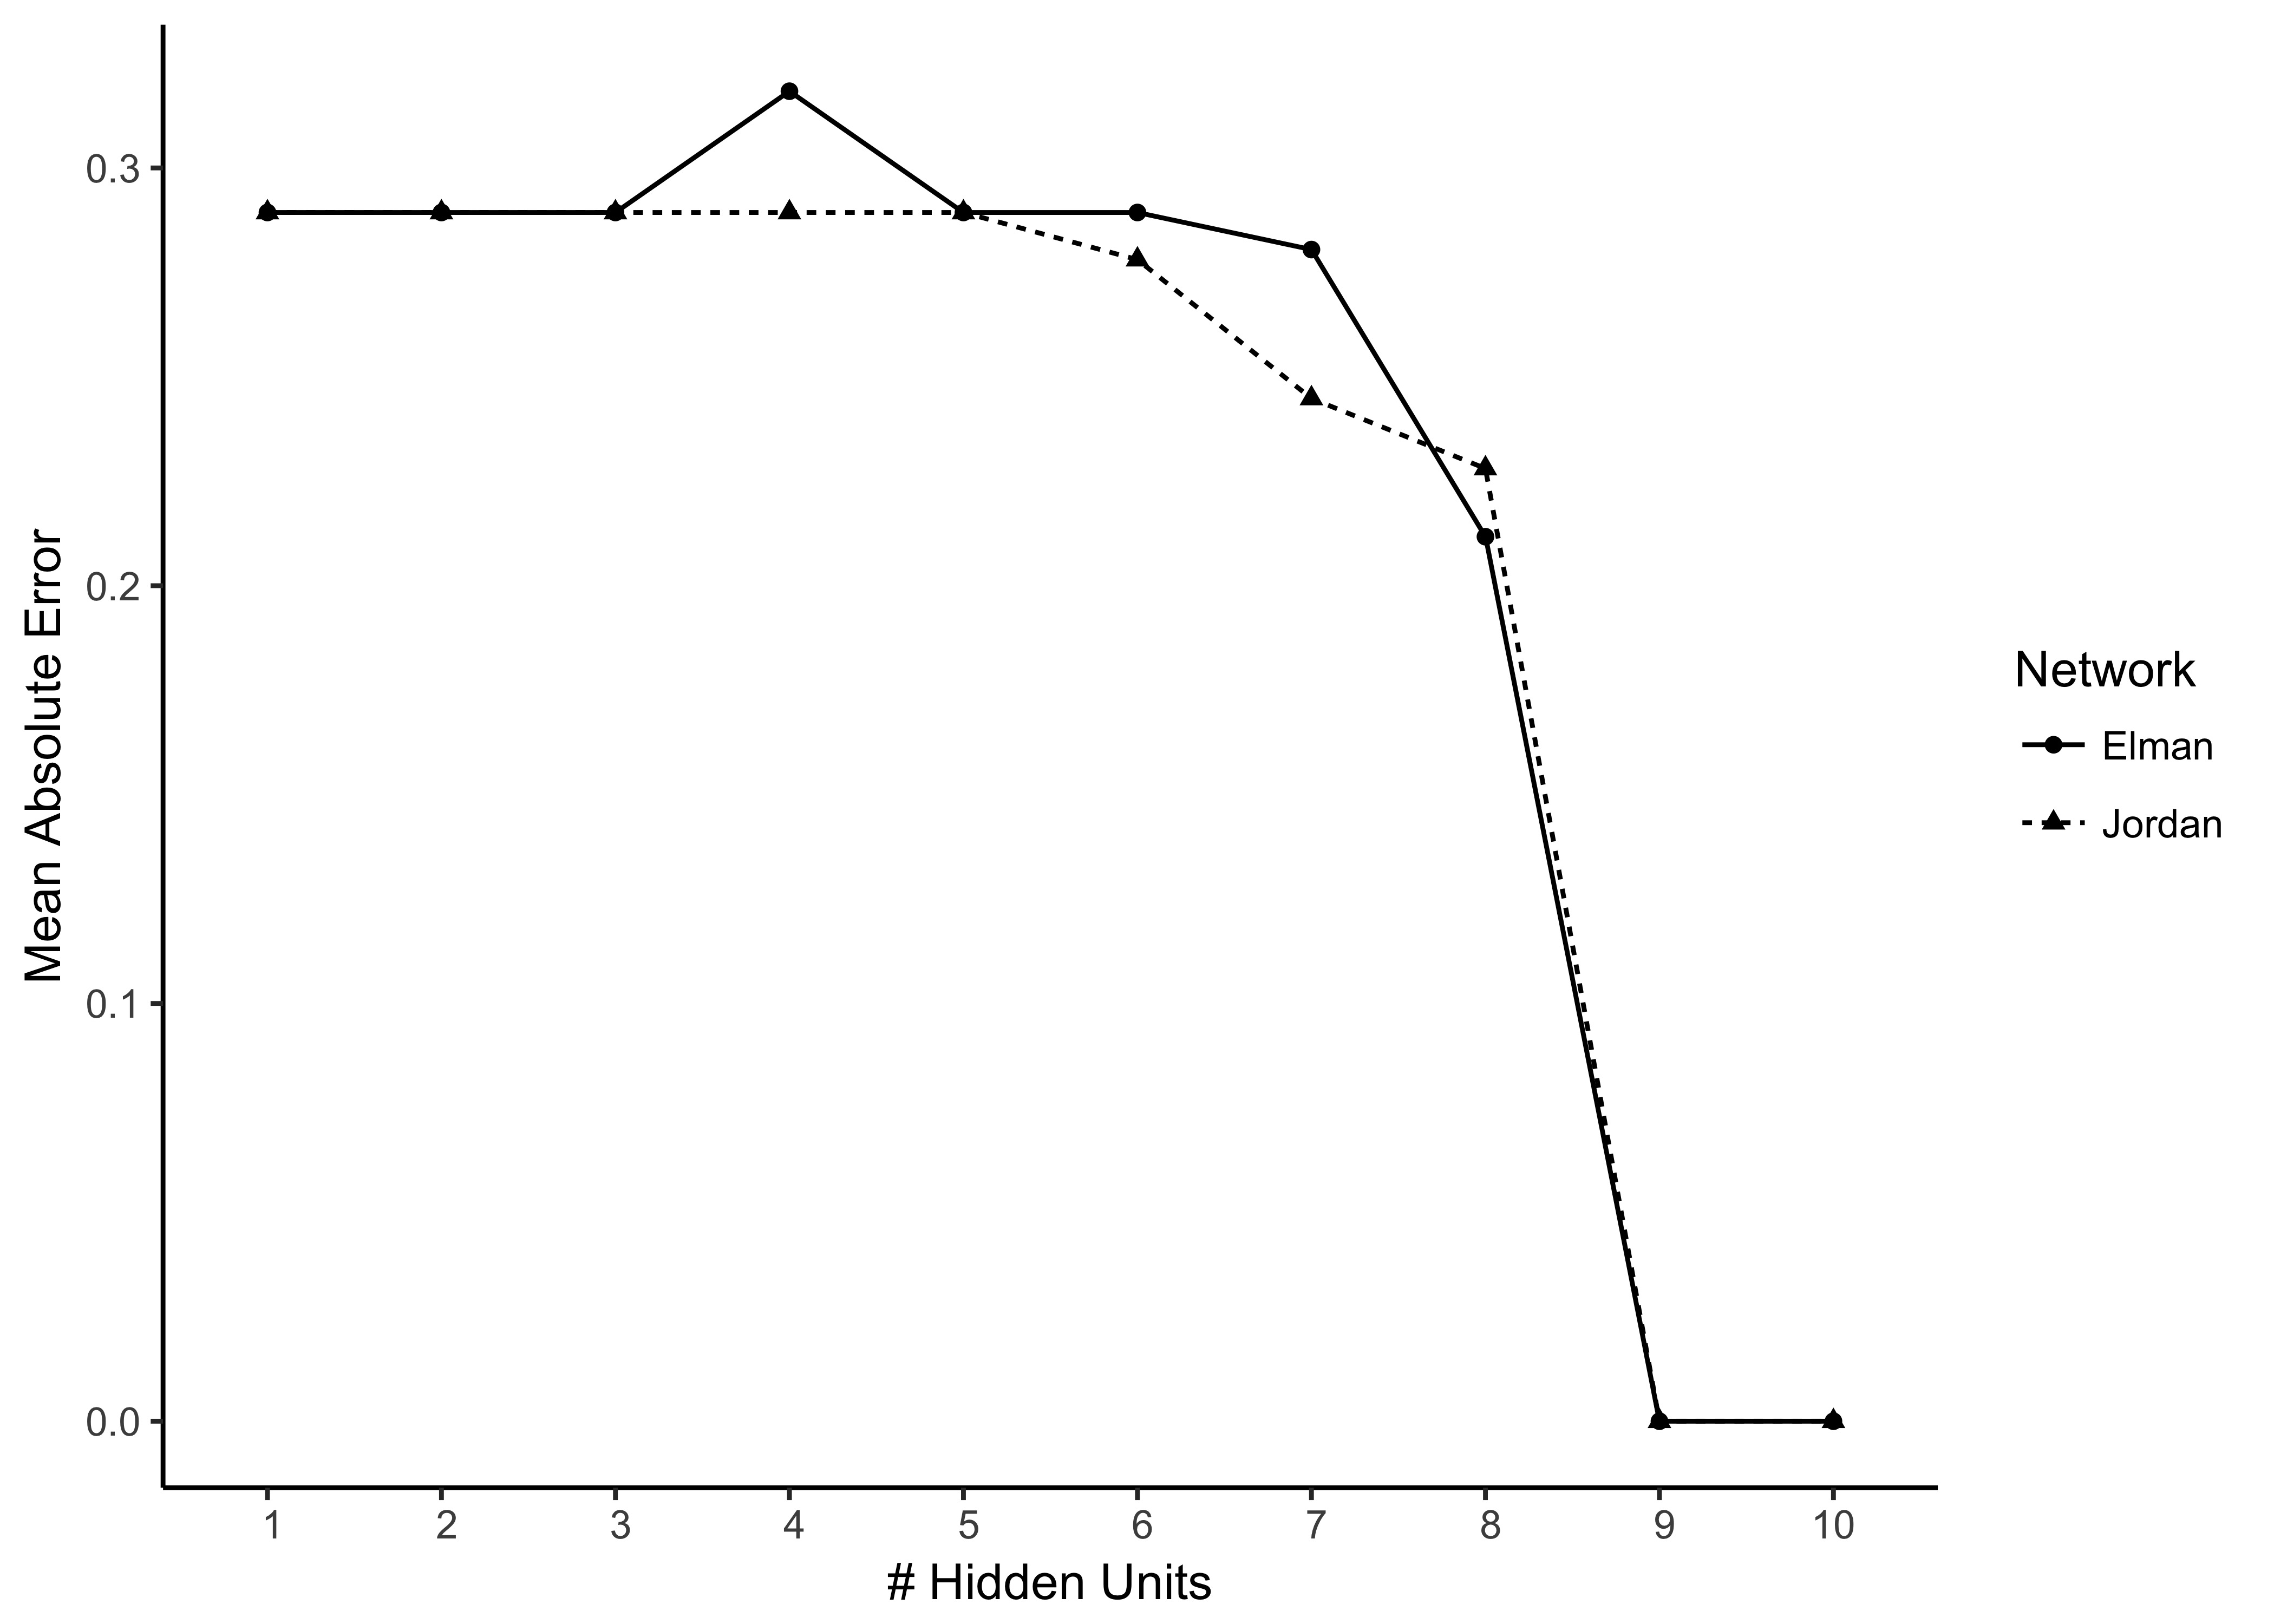
\includegraphics[width=1.0\textwidth]{figures/error_nc_4}
	\caption{Results of an experiment to define the appropriated number of hidden units in a recurrent network to generate non-complementary candidates explanations for the program $\CalP_{sup}$. The size of the hidden units vary from one to ten. The graph plots the mean absolute error (MAE) for a 10-fold cross-validation averaged over ten trials for each network configuration.}
	\label{fig:error_nc_4}
\end{figure}

With this we can conclude that both a Jordan and an Elman network constructed in the way described above have one hundred percent of accuracy for the task of generating all the possible non-complementary candidate explanations for the program $\CalP_{sup}$ and its respective set of abducibles $\CalA_{\CalP_{sup}}$. Although we have focused on showing the results for the set of abducibles $\CalA_{\CalP_{sup}}$, it is easy to observe that the experiment can be repeated in the exact same way for any set of abducible which has cardinality four. The only difference is on which abducible each of the four bits represent which in our case was $e^\top$, $e^\top$, $e^\top$, and $e^\top$, but the representation can easily be substituted by any other set of abducibles without affecting the procedure.

Moreover, as it is shown in the algorithms presented earlier, the process is specified in an abstract level such that it should work for a given set of abducibles of any size. Therefore, we would like to abstract from the previous example and show how one could follow the same steps for any other program with corresponding set of abducibles of different sizes. For this purpose, consider an arbitrary program $\CalP$ and its corresponding set of abducibles $\CalA_\CalP$, where |$\CalA_\CalP$| = N. Both the input and output layers would consist of N+1 units. As explained previously, the ideal number of hidden units can vary from case to case and one way to define this if by reproducing the same experiment developed above. Both the Jordan and Elman networks can be structured in the same way, with the difference on the recurrent connections only.

To show that this is indeed the case we will reproduce the experiment and analyse its output for other values of N. In order to do so, we will show example of programs which have a respective size of abducibles of size N. However, note that, just as we have explained earlier, the programs are only for illustrative purpose but the results shown here can be generalised for any set of abducibles of corresponding cardinality~N. Consider the variations of program $\CalP_{sup}$ shown in Example~\ref{example:suppressionvariation} on page~\pageref{example:suppressionvariation}.

A network that sequentially generates the candidate explanations in $\CalC_{\CalA_{\CalP_{sup'}}}$ consists of three input units and three output units. In order to define the adequate number of units in the hidden layer, we reproduce the experiment for Jordan and Elman networks now following the configurations described here. As it is shown in Figure~\ref{fig:error_nc_2}, again the Jordan and the Elman networks have presented a similar behaviour and a hidden layer consisting of four units seems to be the most adequate for both types of networks. For the candidate explanations $\CalC_{\CalA_{\CalP_{sup''}}}$, the network consists of seven input units and seven output units. Regarding the hidden units, as it is shown in Figure~\ref{fig:error_nc_6}, the Jordan and Elman networks need thirteen and fourteen hidden units, respectively. This last case is also a strong indication on the generalisation capacity of such networks, since there are twenty-seven candidate explanations and less than the half of this number is needed in hidden units.

With this we can conclude that creating Jordan and Elman networks for the generation on non-complementary candidate explanations can be done for sets of abducibles of different sizes by following the steps defined in this section. Moreover, the experiment to define which of the two networks is more suitable and which is the most adequate number of hidden units can also easily be reproduced for the different sets of abducibles. 

\vspace*{\fill}
\begin{tcolorbox}
\begin{example}
\label{example:suppressionvariation}
\normalfont 
Consider a subset $\CalP_{sup'}$ of the program $\CalP_{sup}$ only consisting of the following two clauses:
\[
\begin{array}{lclclcl}
l &\leftarrow& e \wedge \neg ab_1. &\quad\quad& ab_1 &\leftarrow& \bot.
\end{array}
\]
The repesctive set of abducibles $\CalA_{\CalP_{sup'}}$ consists of the following fact and assumption:
\[
\begin{array}{lclclcl}
e &\leftarrow& \top. &\quad\quad& e &\leftarrow& \bot.
\end{array}
\]
The set of non-complementary candidate explanations $\CalC_{\CalA_{\CalP_{sup'}}}$ consists of the following three elements:
\[
\begin{array}{lclclclclcl}
\CalC_0 &=& \emptyset, &\quad& \CalC_1 &=& \{e \leftarrow \top\}, &\quad& \CalC_2 &=& \{e \leftarrow \bot\}.
\end{array}
\]

Consider a program $\CalP_{sub''}$ which is the program $\CalP_{sup}$ with an additional clause, e.g. \textit{if she has a presentation to prepare, then she will study late in the library}. Thus, we have the program $\CalP_{sub''}$ consisting of all the four clauses in $\CalP_{sup}$ plus the following two:
\[
\begin{array}{lclclcl}
l &\leftarrow& p \wedge \neg ab_3. &\quad& ab_3 &\leftarrow& \bot.\\
\end{array}
\]
Where the new atom $p$ stands for \textit{she has a presentation to prepare} and $ab_3$ for the abnormality, as usual. Its repesctive set of abducibles $\CalA_{\CalP_{sup''}}$ consists of the following six elements:
\[
\begin{array}{ccccc}
e \leftarrow \top. & \quad & t \leftarrow \top. & \quad & p \leftarrow \top. \\
e \leftarrow \bot. & \quad & t \leftarrow \bot  & \quad & p \leftarrow \bot.
\end{array}
\]

The set of non-complementary candidate explanations $\CalC_{\CalA_{\CalP_{sup''}}}$ consists of the following twenty seven elements:
\[
\begin{array}{lclclcl}
\CalC_1&=&\emptyset, &&&& \\
\CalC_2 &=& \{e \leftarrow \top\}, && \CalC_3 &=& \{e \leftarrow \bot\}, \\
\CalC_4 &=& \{t \leftarrow \top\}, && \CalC_5 &=& \{t \leftarrow \bot\}, \\
\CalC_6 &=& \{p \leftarrow \top\}, && \CalC_7 &=& \{p \leftarrow \bot\}, \\
\CalC_8 &=& \{e \leftarrow \top, t \leftarrow \top\}, && \CalC_9 &=& \{e \leftarrow \top, t \leftarrow \bot\}, \\
\CalC_{12} &=& \{e \leftarrow \bot, t \leftarrow \top\}, && \CalC_{13} &=& \{e \leftarrow \bot, t \leftarrow \bot\}, \\
 \CalC_{14} &=& \{e \leftarrow \bot, p \leftarrow \top\}, && \CalC_{15} &=& \{e \leftarrow \bot, p \leftarrow \bot\}, \\
\CalC_{16} &=& \{t \leftarrow \top, p \leftarrow \top\}, && \CalC_{17} &=& \{t \leftarrow \top, p \leftarrow \bot\}, \\
\CalC_{18} &=& \{t \leftarrow \bot, p \leftarrow \top\}, && \CalC_{19} &=& \{t \leftarrow \bot, p \leftarrow \bot\}, \\
\CalC_{20} &=& \{e \leftarrow \top, t \leftarrow \top, p \leftarrow \top\}, && \CalC_{21} &=& \{e \leftarrow \top, t \leftarrow \top, p \leftarrow \bot\}, \\
\CalC_{22} &=& \{e \leftarrow \top, t \leftarrow \bot, p \leftarrow \top\}, && \CalC_{23} &=& \{e \leftarrow \top, t \leftarrow \bot, p \leftarrow \bot\}, \\	     
\CalC_{24} &=& \{e \leftarrow \bot, t \leftarrow \top, p \leftarrow \top\}, && \CalC_{25} &=& \{e \leftarrow \bot, t \leftarrow \top, p \leftarrow \bot\}, \\	
\CalC_{26} &=& \{e \leftarrow \bot, t \leftarrow \bot, p \leftarrow \top\}, && \CalC_{27} &=& \{e \leftarrow \bot, t \leftarrow \bot, p \leftarrow \bot\}. 	
\end{array}
\]
\end{example}
\end{tcolorbox}
\vspace*{\fill}

\begin{figure}
	\centering
	\begin{subfigure}[b]{1.\textwidth}
	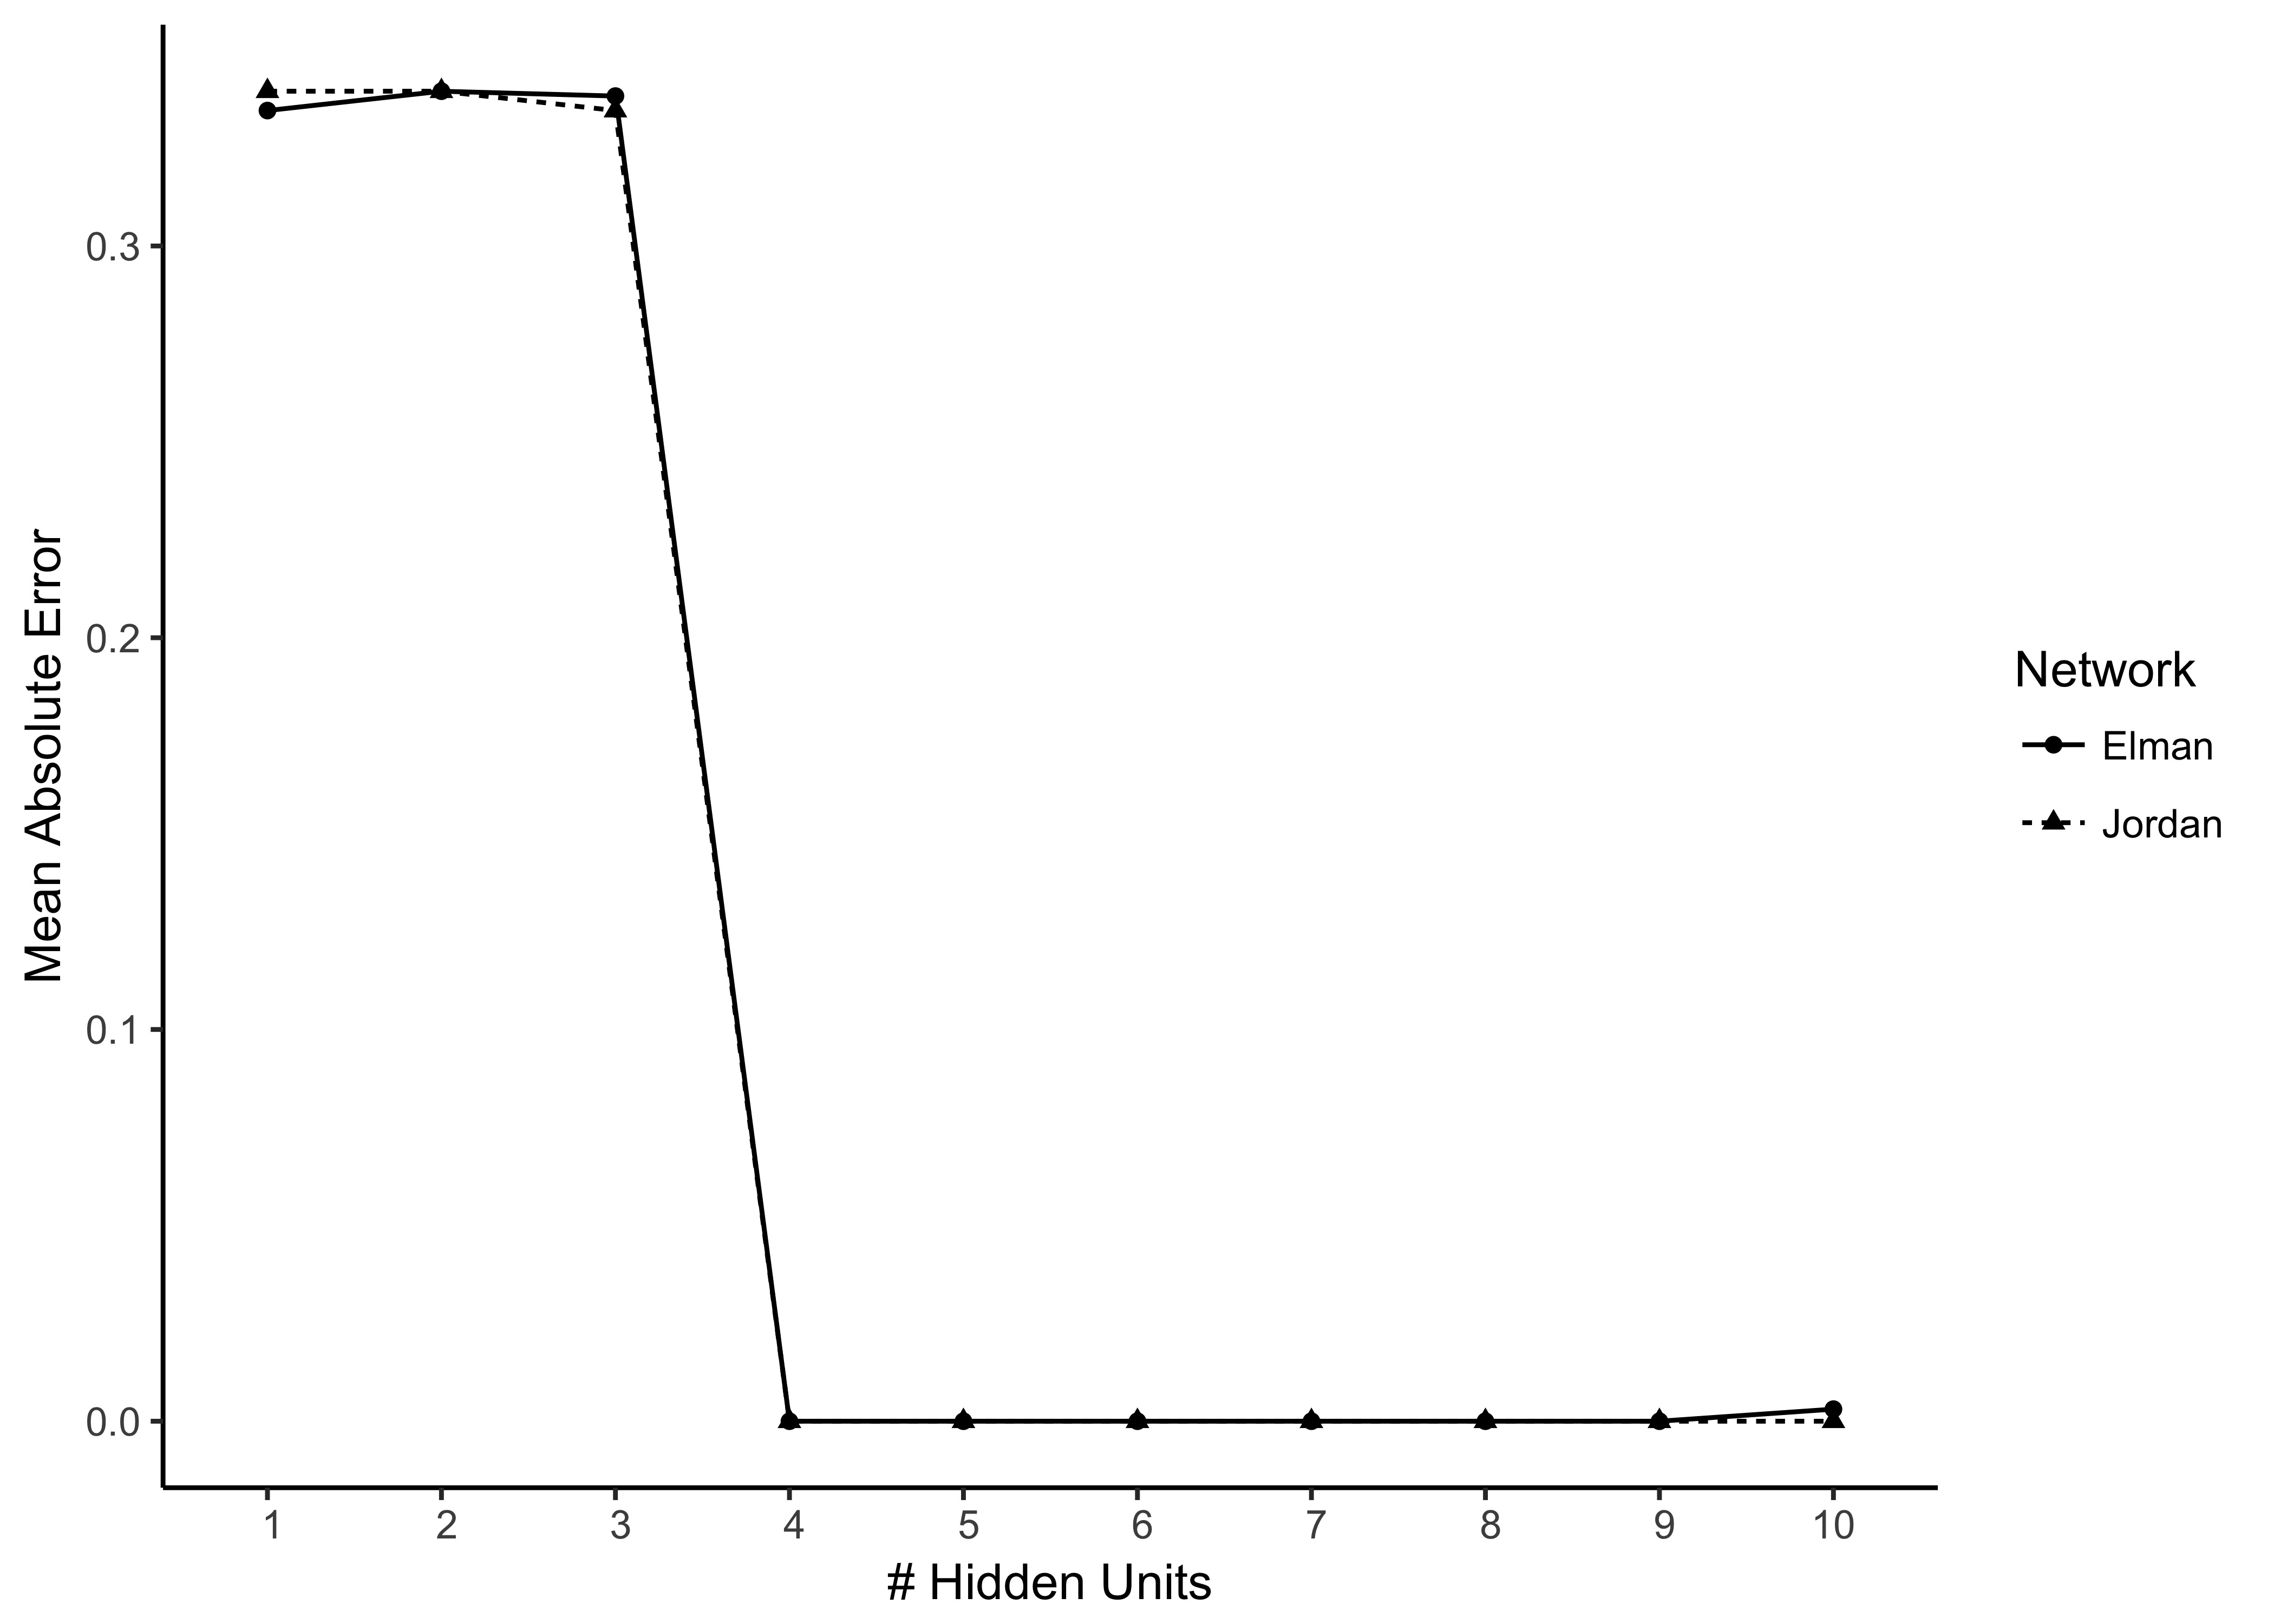
\includegraphics[width=0.9\textwidth]{figures/error_nc_2}
	\caption{Set of abducibles of cardinality two.}
	\label{fig:error_nc_2}
	\end{subfigure}
	\bigskip
	\begin{subfigure}[b]{1.0\textwidth}
  	 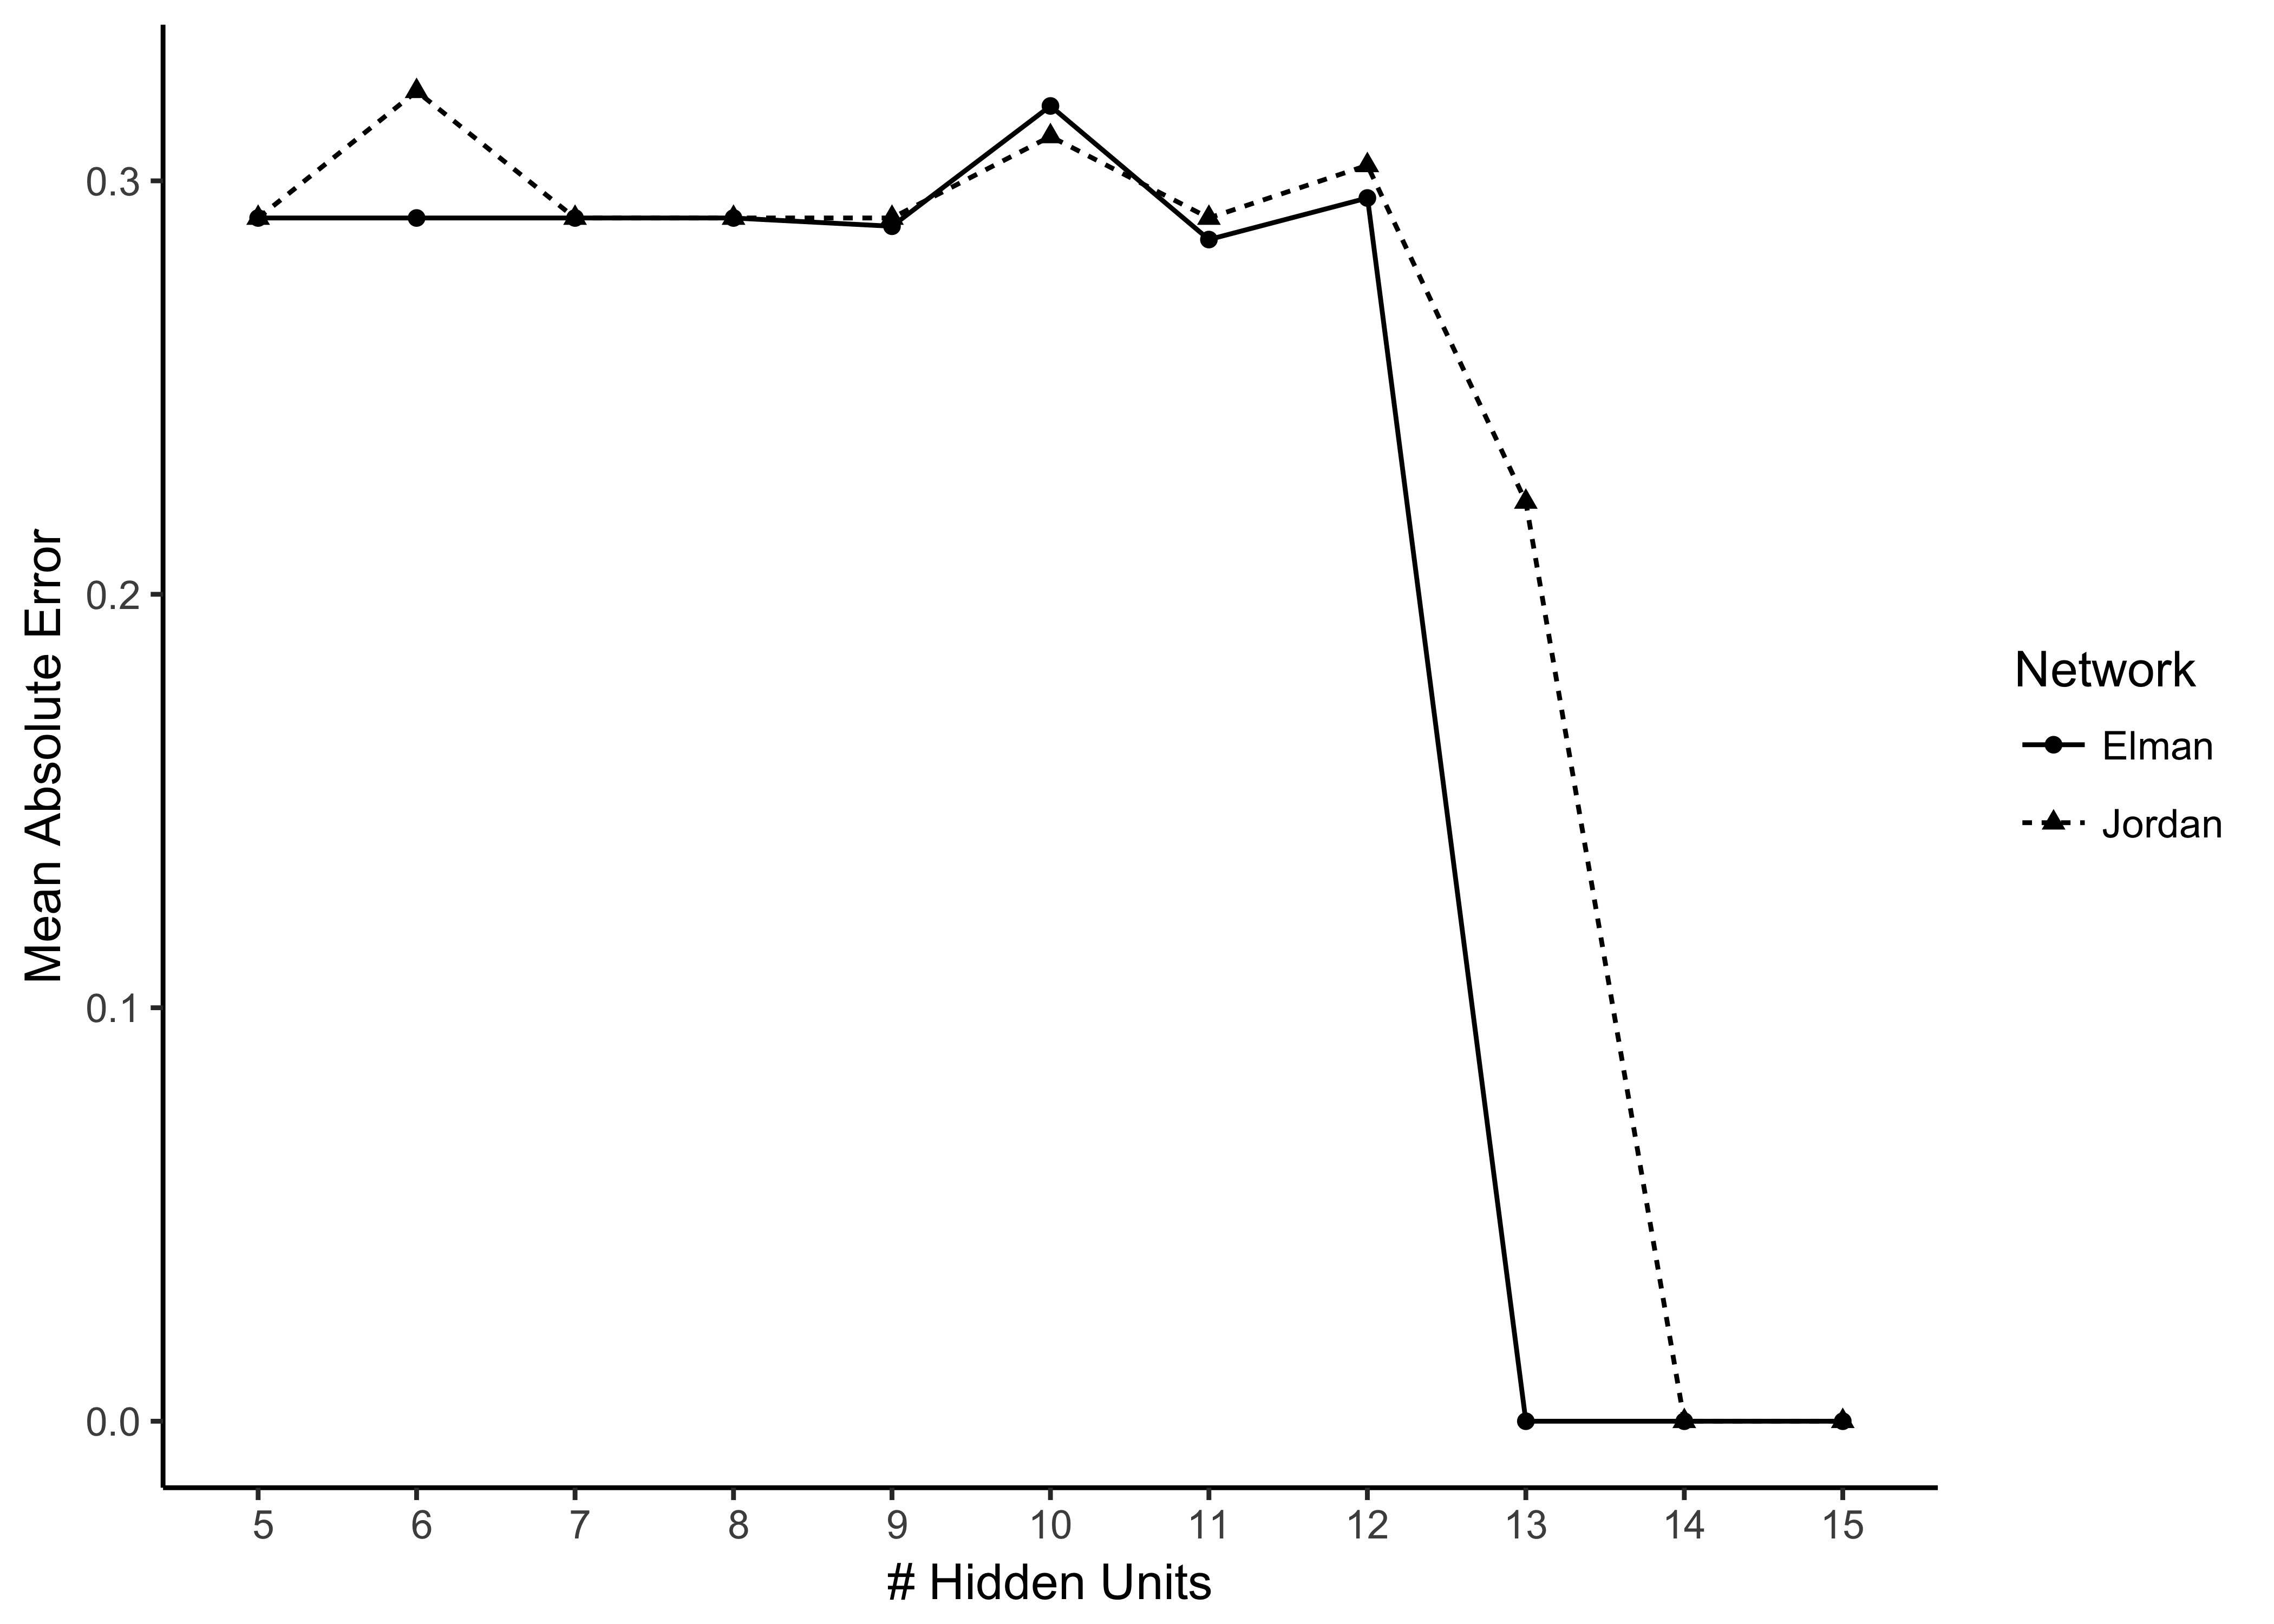
\includegraphics[width=0.9\textwidth]{figures/error_nc_6}
	 \caption{Set of abducibles of cardinality six.}
	\label{fig:error_nc_6}
	\end{subfigure}
	\caption{Results of an experiment to define the appropriated number of hidden units in a recurrent network to generate non-complementary candidates explanations for a given set of abducibles with cardinality two (a) and six (b). The size of the hidden units vary from one to ten. The graph plots the mean absolute error (MAE) for a 10-fold cross-validation averaged over ten trials for each network configuration.}
\end{figure}

Remember that for a set of abducibles $\CalA_\CalP$ of cardinality $2n$, there are $3^n$ non-complementary candidate explanations $\CalC_{\CalA_\CalP}$. These $3^n$ candidates can be ordered as $3^n!$ different sequences. For example, in the most basic case which is $n = 1$, we have that cardinality of $\CalA_\CalP$ is two, there are three candidate explanation which can be ordered in six different sequences, i.e.
\[
\begin{array}{lclclcl}
\CalC_{\CalA_\CalP}^1 &=& \{\CalC_1, \CalC_2, \CalC_3\}, &\quad& \CalC_{\CalA_\CalP}^2 &=& \{\CalC_1, \CalC_3, \CalC_2\},\\
\CalC_{\CalA_\CalP}^3 &=& \{\CalC_2, \CalC_3, \CalC_1\}, &\quad& \CalC_{\CalA_\CalP}^4 &=& \{\CalC_2, \CalC_1, \CalC_3\},\\
\CalC_{\CalA_\CalP}^5 &=& \{\CalC_3, \CalC_1, \CalC_2\}, &\quad& \CalC_{\CalA_\CalP}^6 &=& \{\CalC_3, \CalC_2, \CalC_1\}.
\end{array}
\]

Similarly, there are several different sequences for the sets of non-complementary candidate explanations regarding different cardinalities of the abducibles. In order to train the network with this different orders, we only have to set up the parameter \textit{candidates} in the algorithms shown earlier and everything else works in the same way.

For instance, when solving Byrne's selection task represented by $\CalP_{sup}$, we have used the same sequence from Chapter~\ref{sec:cn} for sake of simplicity. However, any other sequence could have been used, e.g.
\[
\begin{array}{lcl}
candidates^1 &=& \{00000, 10100, 10000, 01000, 00100, 00010, 10010, 01100, 01011\}, \\
candidates^2 &=& \{00000, 10100, 01011, 10000, 01000, 00100, 00010, 10010, 01100\}, \\
candidates^3 &=& \{00000, 10100, 10010, 10000, 01000, 00100, 00010, 01100, 01011\},  \\
candidates^4 &=& \{00000, 00100, 10010, 10000, 01000, 10100, 00010, 01100, 01011\},  \\
\dots\\
candidates^{9!} &=& \{00100, 00010, 01100, 01011, 10100, 10010, 10000, 01000, 00000\}. 
\end{array}
\]

This shows that not only the same result as the one from the previous approach can be archived, but also that arbitrary sequences can be easily considered. However, as explained before, generating the non-complementary candidate explanations is not our main goal. Thus, we will now show how the same networks can also be used to generate the minimal candidate explanations.


\section{Minimal Candidate Explanations}
\label{sec:nn:mce}

In this section will show that recurrent networks can be used not only to generate the non-complementary candidate explanations, as shown in Section~\ref{sec:nn:ncce}, but also to generate the minimal candidate explanations for a given observation. The most important information necessary for this modification is whether the last candidate explanation has in fact explained the given observation or not.  

We again show that this is indeed the case by means of an example. Thus, reconsider the program $\CalP_{sup}$ from Example~\ref{example:suppression} on page~\pageref{example:suppression}. The only necessary modification in the structure of the Jordan and Elman networks presented in Section~\ref{sec:nn:ncce} is to add one bit in the input vector which will now consist of six bits instead of five. This new bit gives us the informations of whether the last candidate was an explanation or not. This is reflected in the network by an additional unit in the input layer. The new version of both networks is shown in Figure~\ref{fig:rnnmin}.

The activation of this new unit $e$ (\textit{explanation}) is done by the external network responsible for checking whether a candidate explanation has explained the given observation or not. This is the same network which activates the unit \textit{next} (\textit{next}), which means that the request of a new candidate explanation and the activation of unit $e$ are synchronised.

\begin{figure}
\centering
   \begin{subfigure}[b]{0.55\textwidth}
   \scalebox{0.7}{\jordanmin}
   \caption{Jordan Network.}
   \bigskip
\end{subfigure}
\begin{subfigure}[b]{0.55\textwidth}
   \scalebox{0.7}{\elmanmin}
   \caption{Elman Network.}
\end{subfigure}
\caption{Structure of the Jordan (a) and Elman (b) networks for the generation of all non-complementary candidate explanations for the program $\CalP_{sup}$. Solid lines are trainable.}
\label{fig:rnnmin}
\end{figure}

Also reconsider the observation 
\[
\CalO_1 = \{l\},
\] 
we know that its minimal explanations given program $\CalP_{sup}$ and the observation $\CalO_1$ are the following:
\[
\begin{array}{lcl}
\CalE_1 &=& \{e \leftarrow \top\}, \\
\CalE_2 &=& \{t \leftarrow \top\}.
\end{array}
\]
Thus, when generating the candidate explanations, all the supersets of the two explanations $\CalE_1$ and $\CalE_2$ should not be taken into account. Thus, if we are also considering that the candidate explanations will be generated following the same order as in the previous sections, the following candidates explanations are expected to be generated: 
\[
\begin{array}{lcl}
\CalE_0 &=& \emptyset,\\
\CalE_1 &=& \{e \leftarrow \top\}, \\
\CalE_2 &=& \{e \leftarrow \bot\}, \\
\CalE_3 &=& \{t \leftarrow \top\}, \\
\CalE_4 &=& \{t \leftarrow \bot\}, \\
\CalE_8 &=& \{e \leftarrow \bot, t \leftarrow \bot\}. 
\end{array}
\]

In terms of the 5-bit binary vectors corresponding to the expected output the expected sequence if we have the next unit activated for six time steps in a row would be: 
\[
00000, 10000, 01000, 00100, 00010, 01011. 
\]
But of course, just as we had before, this is not always the case and, depending on the activation of the next unit, any sequence of the following form would be valid: 
\[
(00000)^+, (10000)^+, (01000)^+, (00100)^+, (00010)^+, (01011)^+.
\]
All possible inputs and its respective expected outputs for this example is shown in Table~\ref{table:inoutmin}. 

\begin{table}
	\centering
	\begin{subtable}[h]{0.30\textwidth}
		\centering
		\begin{tabular}{cc}
		Input & Output \\
		\hline
		000000 & 00000 \\
		100001 & 10000 \\
		010000 & 01000 \\
		001001 & 00100 \\
		000100 & 00010 \\
		010100 & 01011 \\
		\end{tabular}
		\bigskip
		\caption{Cases where the fifth bit in the input is \textit{zero}}
		\label{table:trainingexplanations:zero}
	\end{subtable}
	\hspace{3cm}
	\begin{subtable}[h]{0.30\textwidth}
		\centering
		\begin{tabular}{cc}
		Input & Output \\
		\hline
		000010 & 10000 \\
		100011 & 01000 \\
		010010 & 00100 \\
		001011 & 00010 \\
		000110 & 01011 \\
		010110 & 00000 \\
		\end{tabular}
		\bigskip
		\caption{Cases where the fifth bit in the input is \textit{one}}
		\label{table:trainingexplanations:one}
	\end{subtable}
	\caption{Each possible input and its respective expected output for the generation of minimal candidate explanations for the program $\CalP_{sup}$ and observation $\CalO_1 = \{l\}$ considering a specific ordering.}
	\label{table:inoutmin}
\end{table}

Note that, when we assume the candidates to be minimal, there is a cardinality constraint implicit in the ordering of the candidates. For the program $\CalP_{sup}$ which we are discussing, for example, the following ordering could no longer be considered: 
\[
\begin{array}{lcl}
candidates^2 &=& \{00000, 10100, 01011, 10000, 01000, 00100, 00010, 10010, 01100\}.
\end{array}
\]
The candidate explanation $10100$ representing $\{e^\top, t^\top\}$ is a positive non-minimal candidate explanation which the generation could not have been avoided if this order is considered. Therefore, we assume that for the generation of minimal candidate explanations, the sequences will respect the cardinality order. However, this does not mean that the order is now fixed. For a given set of candidates $\CalC$, there are the following number of sequences respecting the cardinality constraint:
\[
c_0! * c_1! * \dots * c_n!
\]
where $c_i$ represents the number of candidates in $\CalC$ with cardinality $i$. In our example, the six minimal candidates can be ordered as
\[
1!*4!*1! = 16
\]
different sequences, as there is one candidate with cardinality zero, four with cardinality one and one with cardinality two.

The training and the testing phase of the Jordan and Elman networks are done in the same way as described before. The only difference now is in the input of the network and the training and testing data. The input of the network will now contain an aditonal bit representing the request of next candidate explanation. The data will now be generated considering all the possibilities of candidates being explanations and the resulting minimal set of candidate explanations for each of this cases. Table~\ref{table:inoutmin} shows one of this potential cases for a given program having a correspondent set of abducibles of size four.

As we know that in the case where the fifth bit is zero only the identity function is computed, we will only consider the cases where the fifth bit is one to demonstrate all the possible sixteen sequences for potential programs $\CalP$ and observations $\CalO$, such that the set of abducibles $\CalA_\CalP$ has cardinality four. Figure~\ref{fig:exptree} on page~\pageref{fig:exptree} shows all the possible outcomes and paths for each of these cases and Table~\ref{table:allinoutmin} shows the data we use in the training process such that the Jordan and Elman networks can reflect this behaviour.

So the new training and testing data for a given program $\CalP$ with a respective set of abducibles $\CalA_\CalP$ of size four will not only have a fixed sequence of size nine being generated, but all the ten different sequences of different sizes. This different sequences are due to the possible variations in the activation of unit $e$. We assume a corresponding program and observation which which leads to these expected data can be easily found. Therefore, in each pass of the training phase as well as in the testing phase, we choose one arbitrary mapping of potential input to expected output from the sixteen shown in Table~\ref{table:allinoutmin} on page~\pageref{table:allinoutmin}.

\begin{table}
	\begin{subtable}[h]{0.10\textwidth}
		\centering
		\begin{tabular}{cc}
		Input & Output \\
		\hline
		000010	&	10000 \\
		100010	&	01000 \\
		010010	&	00100 \\
		001010	&	00010 \\
		000110	&	10100 \\
		1010	10	&	10010 \\
		100110	&	01100 \\
		011010	&	01011 \\
		010110	&	00000 \\
		\end{tabular}
		\bigskip
		%\caption{}
		\label{table:trainingexplanations:zero}
	\end{subtable}
	\hspace{3.75cm}
	\begin{subtable}[h]{0.10\textwidth}
		\centering
		\begin{tabular}{cc}
		Input & Output \\
		\hline
		010110	&	00000\\
		000010	&	10000\\
		100011	&	01000\\
		010010	&	00100\\
		001010	&	00010\\
		000110	&	01100\\
		011010	&	01011\\
		&\\
		&\\
		\end{tabular}
		\bigskip
		%\caption{Cases where the fifth bit in the input is \textit{one}}
		\label{table:trainingexplanations:one}
	\end{subtable}
	\hspace{3.75cm}
	\begin{subtable}[h]{0.10\textwidth}
		\centering
		\begin{tabular}{cc}
		Input & Output \\
		\hline
		100110	&	00000\\
		000010	&	10000\\
		100010	&	01000\\
		010011	&	00100\\
		001010	&	00010\\
		000110	&	10100\\
		1010	10	&	10011\\
		&\\
		&\\
		\end{tabular}
		\bigskip
		%\caption{Cases where the fifth bit in the input is \textit{one}}
		\label{table:trainingexplanations:one}
	\end{subtable}
	\newline
	\begin{subtable}[h]{0.10\textwidth}
		\centering
		\begin{tabular}{cc}
		Input & Output \\
		\hline
		010110	&	00000\\
		000010	&	10000\\
		100010	&	01000\\
		010010	&	00100\\
		001011	&	00010\\
		000110	&	10010\\
		100110	&	01011\\
		\end{tabular}
		\bigskip
		%\caption{Cases where the fifth bit in the input is \textit{one}}
		\label{table:trainingexplanations:one}
	\end{subtable}
	\hspace{3.75cm}
	\begin{subtable}[h]{0.10\textwidth}
		\centering
		\begin{tabular}{cc}
		Input & Output \\
		\hline
		011010	&	00000\\
		000010	&	10000\\
		100010	&	01000\\
		010010	&	00100\\
		001010	&	00010\\
		000111	&	10100\\
		1010	10	&	01101\\
		\end{tabular}
		\bigskip
		%\caption{Cases where the fifth bit in the input is \textit{one}}
		\label{table:trainingexplanations:one}
	\end{subtable}
	\hspace{3.75cm}
	\begin{subtable}[h]{0.10\textwidth}
		\centering
		\begin{tabular}{cc}
		Input & Output \\
		\hline
		010110	&	00000\\
		000010	&	10000\\
		100011	&	01000\\
		010010	&	00100\\
		001011	&	00010\\
		000110	&	01011\\
		\end{tabular}
		\bigskip
		%\caption{Cases where the fifth bit in the input is \textit{one}}
		\label{table:trainingexplanations:one}
	\end{subtable}
	\newline
	\begin{subtable}[h]{0.10\textwidth}
		\centering
		\begin{tabular}{cc}
		Input & Output \\
		\hline
		011010	&	00000\\
		000010	&	10000\\
		100011	&	01000\\
		010010	&	00100\\
		001010	&	00010\\
		000111	&	01101\\
		\end{tabular}
		\bigskip
		%\caption{Cases where the fifth bit in the input is \textit{one}}
		\label{table:trainingexplanations:one}
	\end{subtable}
		\hspace{3.75cm}
		\begin{subtable}[h]{0.10\textwidth}
		\centering
		\begin{tabular}{cc}
		Input & Output \\
		\hline
		100110	&	00000\\
		000010	&	10000\\
		100010	&	01000\\
		010011	&	00100\\
		001011	&	00010\\
		000110	&	10011\\
		\end{tabular}
		\bigskip
		%\caption{Cases where the fifth bit in the input is \textit{one}}
		\label{table:trainingexplanations:one}
	\end{subtable}
	\hspace{3.75cm}
	\begin{subtable}[h]{0.10\textwidth}
		\centering
		\begin{tabular}{cc}
		Input & Output \\
		\hline
		010110	&	00000\\
		000010	&	10000\\
		100010	&	01000\\
		010011	&	00100\\
		001010	&	00010\\
		000111	&	01011\\
		\end{tabular}
		\bigskip
		%\caption{Cases where the fifth bit in the input is \textit{one}}
		\label{table:trainingexplanations:one}
	\end{subtable}
	\newline
	\begin{subtable}[h]{0.2\textwidth}
		\centering
		\begin{tabular}{c|c}
		Input & Output \\
		\hline
		000111	\quad	000111	\quad	000111	\quad	000111	\quad	000111	\quad	000110	\quad	000110    &	00000\\	
		000010	\quad	000010	\quad	000010	\quad	000010	\quad	000010	\quad	000010	\quad	000010	&	10000\\
		100011	\quad	100010	\quad	100010	\quad	100011	\quad	100011	\quad	100011	\quad	100011	&	01000\\
		010011	\quad	010010	\quad	010011	\quad	010010	\quad	010011	\quad	010011	\quad	010011	&	00100\\
		001011	\quad	001011	\quad	001011	\quad	001011	\quad	001010	\quad	001011	\quad	001010	&	00011\\
		\end{tabular}
		\bigskip
		%\caption{Cases where the fifth bit in the input is \textit{one}}
		\label{table:trainingexplanations:one}
	\end{subtable}
	\caption{Input and expected output for all the sixteen possible combinations of the fifth bit representing $explanation$.}
	\label{table:allinoutmin}
\end{table}

The same experiment described in the previous section is then performed again, but now taking into account the modifications in the generation of the training and verification data. In practice, all the algorithms shown before work exactly in the same way with the only difference that instead of having one fixed sequence of candidate explantions to be learned, we now have a set of possible candidate explanations. An arbitrary one is chosen from this set in the beginning of every new training phase.

The performance measure considered is also the same, e.g. mean absolute error. Figure~\ref{fig:error_min_4} on page~\pageref{fig:error_min_4} shows the result of this experiment for the generation of minimal candidate explanation for a given program $\CalP$ with set of abducibles $\CalA_\CalP$ of size four. This network could then be used, for instance, to generate the minimal candidate explanations for a given observation $\CalO$ given the program~$\CalP_{sup}$, since its respective set of abducibles $\CalA_{\CalP_{sup}}$ consists of four facts and assumptions.

If we filter the results shown in Figure~\ref{fig:error_min_4} to see only the mean absolute error with respect to the cases shown in Table~\ref{table:inoutmin} which corresponds to the given observation $\CalO_1$, we get the results shown in Figure~\ref{fig:l_error_min_4} on page~\ref{fig:error_min_4}.

\begin{figure}
	\centering
	\begin{subfigure}[b]{1.\textwidth}
	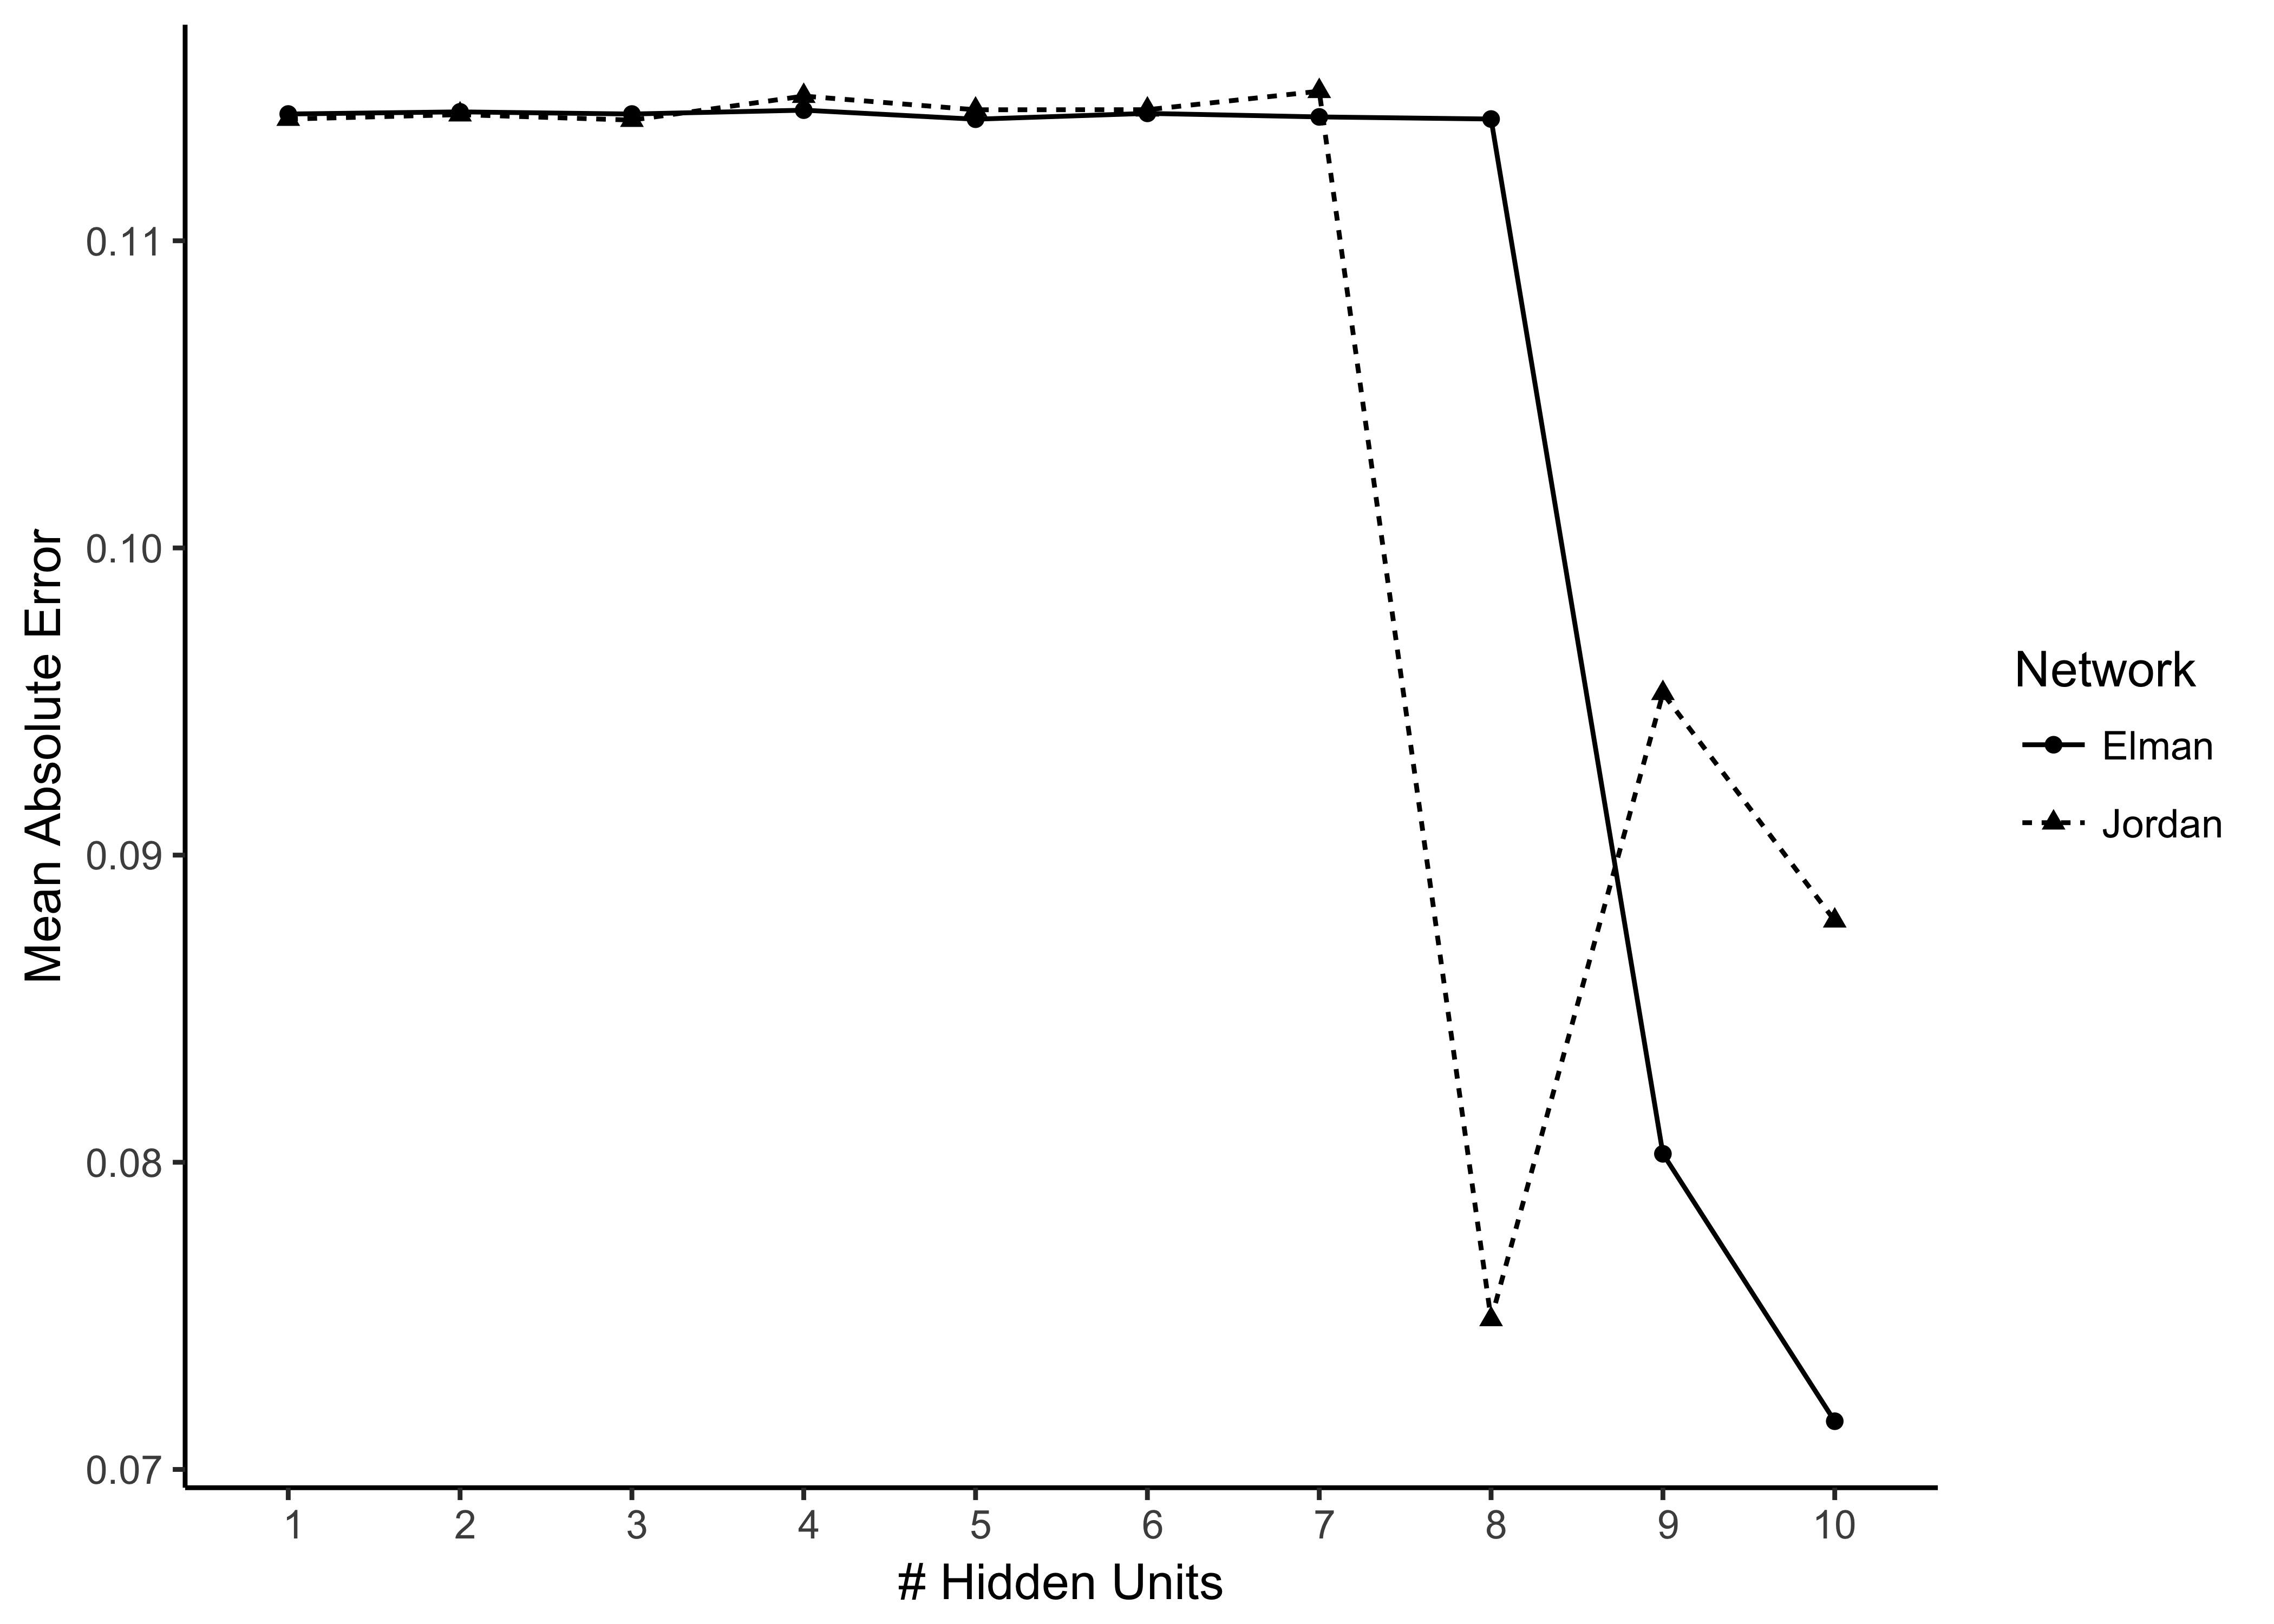
\includegraphics[width=0.9\textwidth]{figures/error_min_4}
	\caption{General results.}
	\label{fig:error_min_4}
	\end{subfigure}
	\bigskip
	\begin{subfigure}[b]{0.9\textwidth}
  	 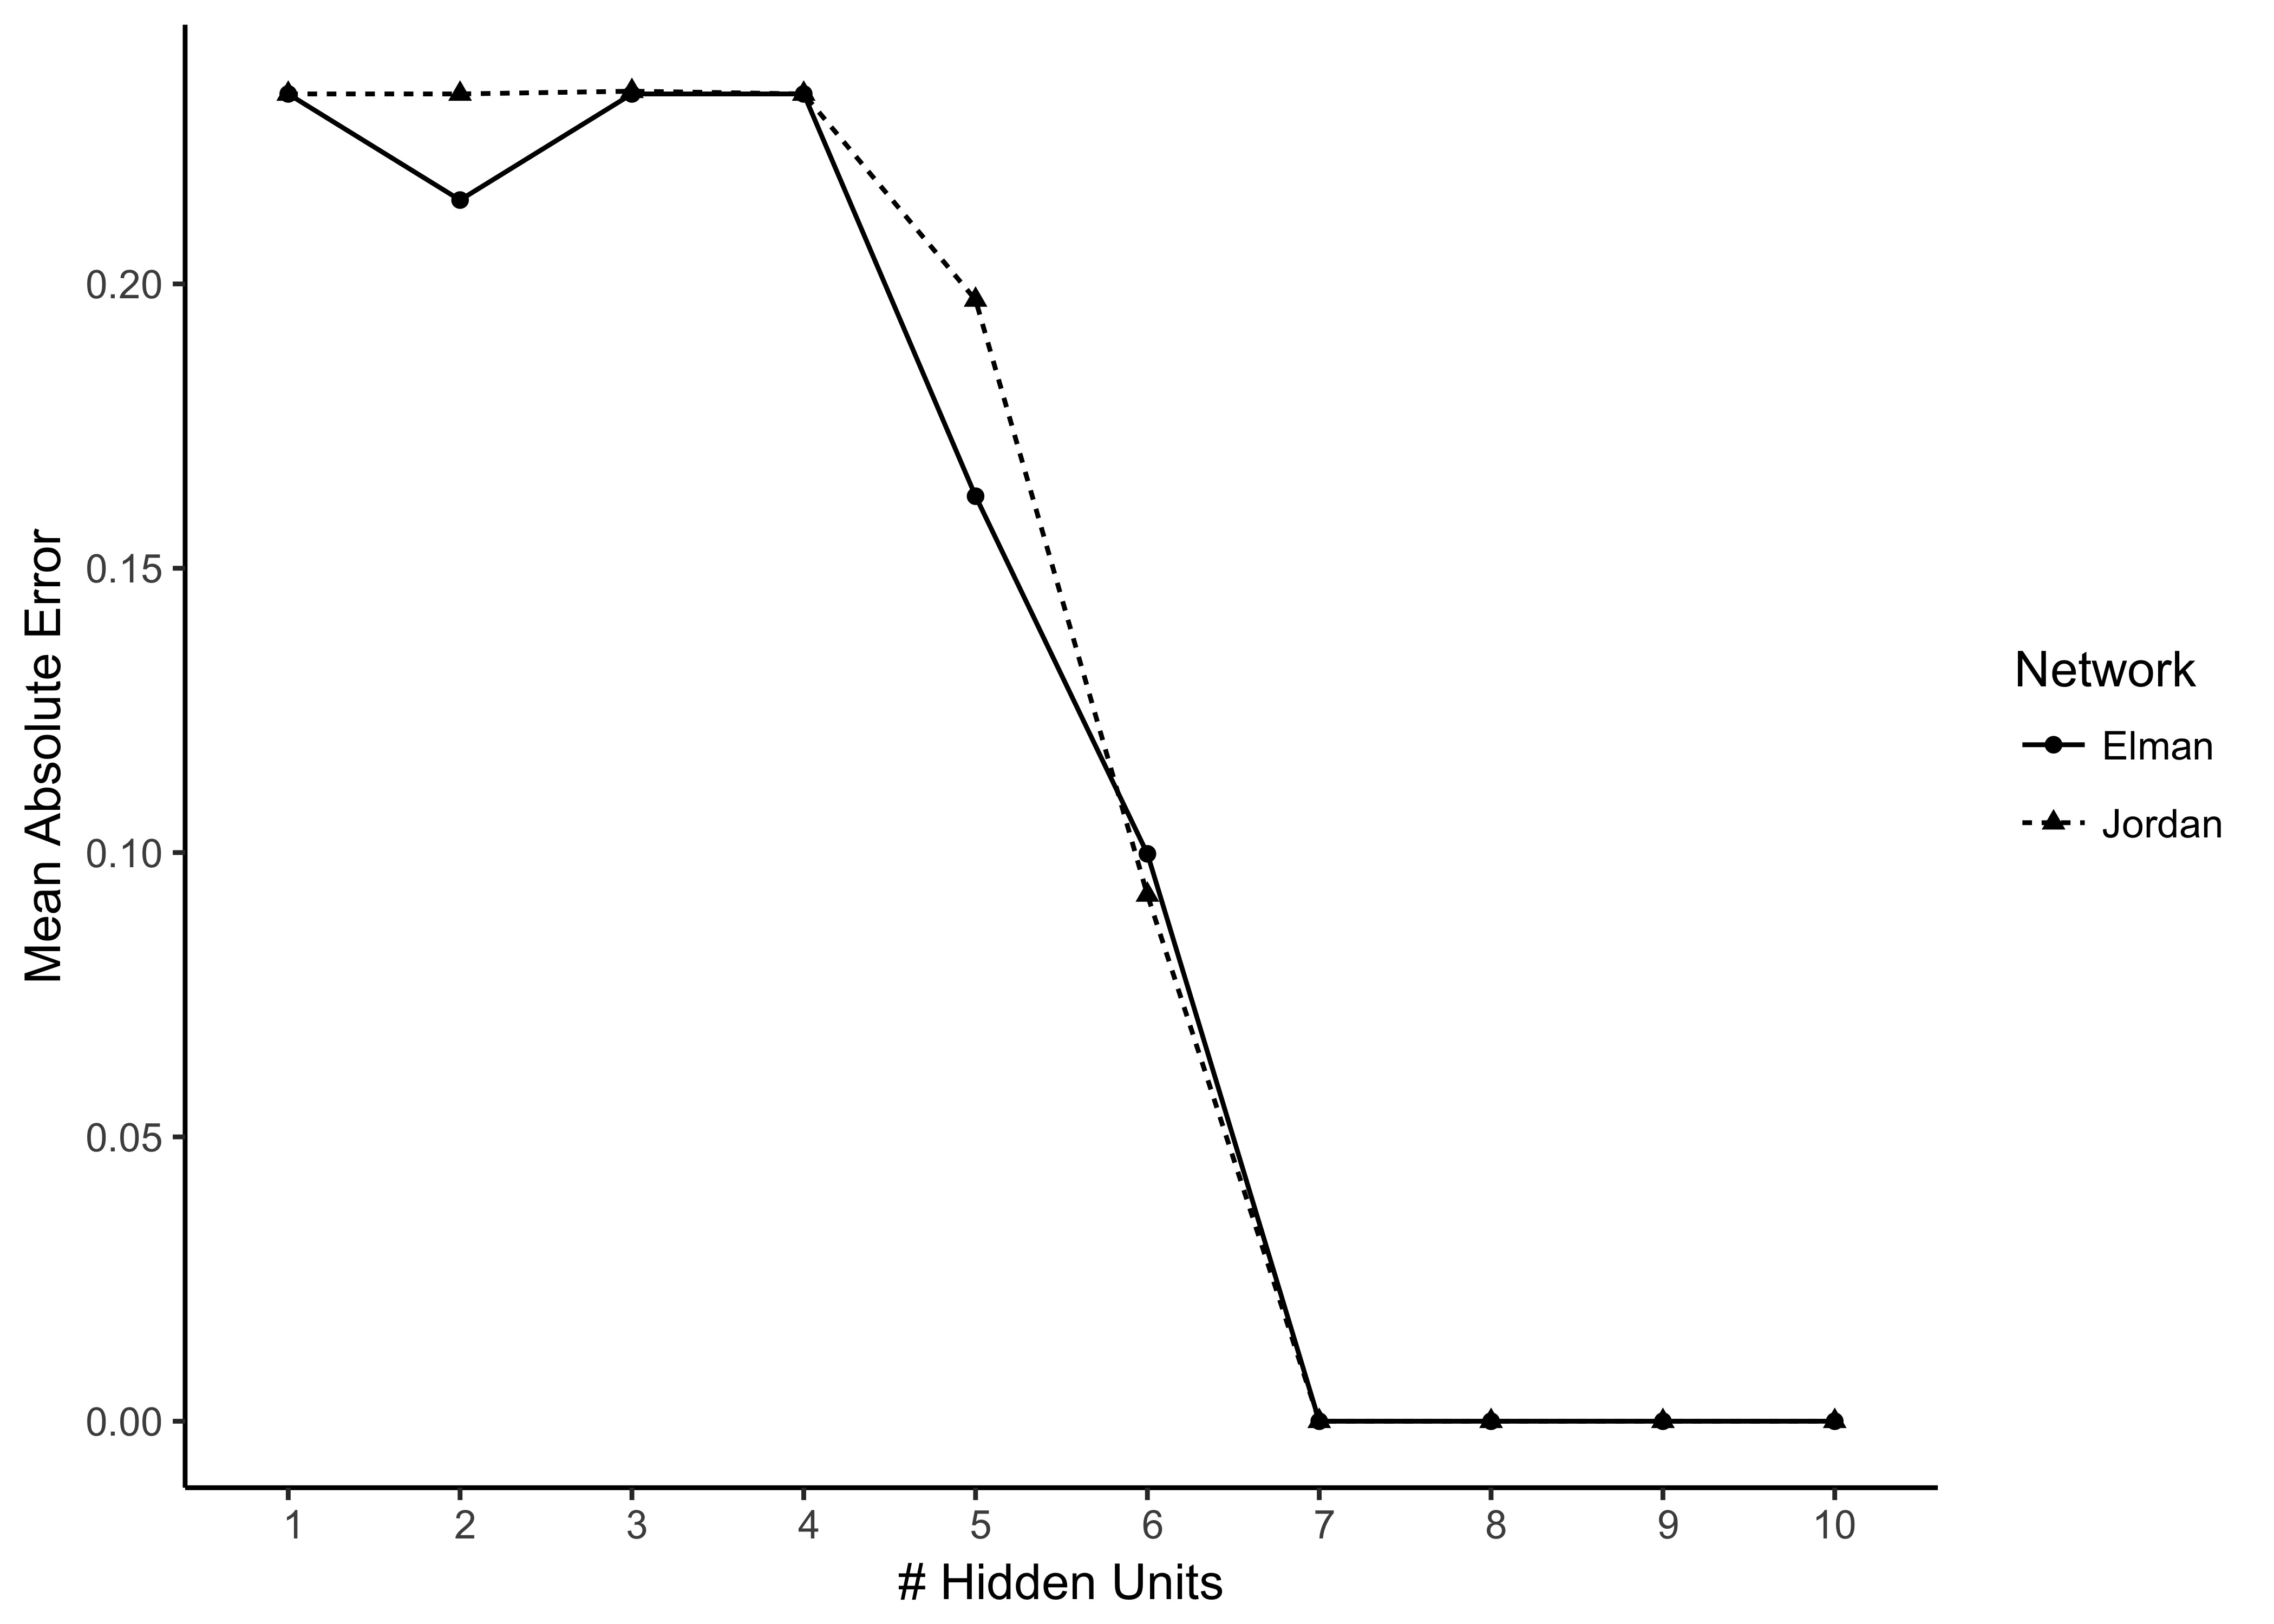
\includegraphics[width=1.0\textwidth]{figures/l_error_min_4}
	 \caption{Results filtrated by the test cases considering program $\CalP_{sup}$ and observation~$\CalO_1$.}
	\label{fig:l_error_min_4}
	\end{subfigure}
	\caption{Results of an experiment to define the appropriated number of hidden units in a recurrent network to generate non-complementary candidates explanations for a set of abducibles of cardinality four, considering arbitrary programs and potential explanations. The size of the hidden units vary from one to ten. The graph plots the mean absolute error (MAE) for a 10-fold cross-validation averaged over ten trials for each network configuration.}
\end{figure}

With this we have shown that the Jordan and Elman networks can also be used to generate only the minimal candidate explanations for observation $\CalO_1$ given program $\CalP_{sup}$ with accuracy of one hundred percent starting from seven hidden units on. 

Let us now consider another observation, e.g.
\[
\CalO_2 = \{\neg l\}
\]
In this case, the only explanation for the observation $\CalO_2$ given the program $\CalP_{sup}$ would be the explanation
\[
\CalE_9 = \{e \leftarrow \bot, t \leftarrow \bot\}.
\]

Therefore, all the nine candidate explanations would be generated just like in the network presented in the previous section, since only the last candidate
\[
\CalC_9 = \CalE_9 = \{e \leftarrow \bot, t \leftarrow \bot\}.
\]
is an explanation for the given observation. However, as we will see later, this is not the case for programs with a larger respective set of abducibles. Moreover, because these networks can easily learn different sequences of candidate explanations, we will all propose some cognitive experiments to define which order is the most appropriate one.

Just like in the previous section, the process shown here for a set of abducible consisting of four facts and assumptions can be easily repeated for sets of abducibles of different cardinalities. The only difference from the previous cases is that now the observation also plays a role in the sequence of candidate explanations to be generated, so even the same program could have different outcomes for different observations. This was illustrated by the example shown earlier.

Concerning the learning of arbitrary sequences of candidate explanations, throughout this section we have assumed a specific order for didactic reasons and to let clear how this networks can simulate the previous approach. However, any of the possible sequences mentioned earlier could have been chosen instead of the one which has been used. In fact, we have also repeated the tests shown in this section considering different orderings for those candidate and the results presented here were not affected.

\section{Conclusion}
\label{sec:elman:conclusion}

In this chapter we have shown how to make use of Jordan and Elman networks to perform the task of generating candidate explanations. We started by defining how the non-complementary candidate explanations can be generated
 and then we restricted this candidates to the minimal ones. We have performed experiments to find the optimal number of hidden units for each of the two cases and also compared the results given by each of the two networks considered here.
 
As one may observe from these results, in all tested cases, there are some small differences on the number of hidden units necessary for the Jordan and Elman networks to perform the task, but, in general, they have shown to perform equally good. Concerning the generalisation capacity of these networks, this characteristic is not clear when considering the sets of the abducibles with small cardinality. However, this already changes for cardinality equals six, where there are twenty-seven candidates to be generated but only thirteen hidden units is enough to perform the task.


Given this, we can conclude that the approach presented in this chapter can perform as good as the one shown in Chapter~\ref{sec:cn} with the advantage that we abstracted the structure of the network. This means that we can generate the same sequence of candidate explanation as before, but with a fixed and well defined structure which can be reused for sets of abducibles of different sizes. In the current approach, instead of constructing a new network from the stretch for each possible cardinality of the set of abducibles, we reuse the same network structure and only have to learn the different sequences for each cardinality.

Moreover, as we have also shown, the process of creating and training such a network to generate the candidate explanations is totally automatised. The only necessary steps are the set up of parameters such as cardinality of the set of abducibles and which network to be used. Besides of this, since the generation of candidates is now done by means of learning, we can easily consider different orders for the sequence of candidates. As we will see later, the order in which the candidates are generated can play a role on the sceptical consequences if we are considering bounded reasoning. This gives our current approach one more advantage over the previous one.
